\section{Introduction}

\subsection{Introduction}

This course is about all the architectural components of a database management system. While the DMDB Bachelor course was mostly about basic, abstract and high-level concepts, this course goes deeper into the importance of the architectural design of a DBMS. This includes principles on how to (efficiently) store data on disk and memory, how to move data from disk to memory, processing and optimizing queries, understanding the underlying concepts of query operators, concurrency control and recovery. Figure \ref{fig:arch} is an overview of the architectural components of a DBMS and for a more detailed graphic refer to Figure \ref{fig:arch2}. Some basic terms are explained in the following few paragraphs.

\begin{figure}[h]
	\centering
	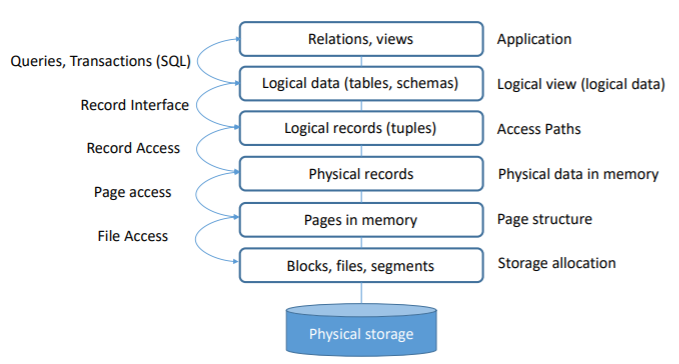
\includegraphics[scale=0.8]{images/00-arch.PNG}
	\caption{Architecture of a DBMS.}
	\label{fig:arch}
\end{figure}

\paragraph{Database Management System (DBMS)}
Tool that helps develop and run data-intensive applications. A DBMS pushes the complexity of dealing with the data (storage, processing, consistency) to the database rather than to the program.

\paragraph{Data Independence}
User applications are immune to changes made in the definition and organization of data. A DBMS provides an abstract view of the data that hides details of data representation and storage.

\paragraph{Logical Data Independence}
The logical structure of data is known as the schema definition (see below). Independence refers to the ability to modify the logical schema without causing application programs to be rewritten. A database allows to build views over the schema s.t. different logical interpretations of the same data are possible. E.g. adding a new column to one user will not change the outcome for another user.

\paragraph{Physical Data Independence}
The ability to modify the physical schema (e.g. to improve performance) without causing the application programs to be rewritten i.e. without affecting the conceptual / external view of the data. The database hides how the data is actually stored persistently and represented in memory.

\paragraph{Schema}
Organization of data, i.e. a blueprint of how the DB is constructed. The formal definition is a set of integrity constraints. In a relational DB, the schema defines elements like tables, fields, relationships views, indexes, etc. The schema is generally stored in a data dictionary. Most common examples include:

\textbf{Flat Model:} Two-dimensional array, elements in each column have the same data type and elements of same row relate to each other. I.e. a single DB table with no relations.

\textbf{Hierarchical Model:} Tree with one-to-many relationships between parent and child nodes. I.e. an XML / JSON file.

\textbf{Network Model:} The above but with many-to-many relationships a.k.a. a graph, potentially with cycles.

\textbf{Relational Model:} We all (should) know what this is.

\textbf{Star Schema:} One or more fact tables (quantitative data) referencing any number of dimension tables (descriptive attributes related to fact data). E.g. a DB of sales: each sale is a fact with date, store, product, etc. and each fact-field is connected to a dimension table that describes that fact field (date dimension would be day, month, year, etc.). A RDBMS can be structured into a star. Mostly used for OLAP. Special Case of a snowflake schema.

\textbf{Snowflake Schema:} Star schema with normalized dimensions, i.e. a single dimension field can be connected to another entire dimension table.

\paragraph{Declarative Language}
SQL is a declarative language and specifies how the result looks like while describing the tuples that should be part of it. A DL does not specify how to get to the result (i.e. no control flow, only logic of a computation - what, not how). With this, the DB can optimize queries.

\paragraph{Function and Data Shipping}
In a distributed system (see parallel architectures below), resources have to be used optimally for efficient query processing. Function shipping refers to processing the data close to where it is actually stored with the results being sent back to the requester. Data shipping refers to moving data to the place where it is processed (as in shared-disk architectures since data needs to be moved from disk to memory to be processed). Both concepts can be combined (as in shared-nothing architectures).


\subsection{Reading Assignments}

For this section, there is only one reading assignment and it is pretty long. It is incredibly helpful though and provides a good overview on almost all the topics discussed in this course. Link \href{https://dsf.berkeley.edu/papers/fntdb07-architecture.pdf}{here}. Most topics are scattered across the next Sections.


\subsubsection{Architecture of a Database System}

\begin{figure}[h]
	\centering
	\includegraphics[scale=0.9]{images/00-arch2.PNG}
	\caption{Main components of an RDBMS.}
	\label{fig:arch2}
\end{figure}

\paragraph{Life of a Query}
We move down and up in the following stack to handle a query:
\begin{enumerate}
    \item Client calls API that communicates over a network to establish a connection with the \textbf{Client Communication Manager}, which responds to SQL commands and returns data / control messages.
    \item The \textbf{Process Manager} assigns a thread of computation to the command if there are enough resources to handle it or delays it until there are.
    \item The \textbf{Relational Query Processor} checks if the user is authorized to run the query, compiles the SQL text to an internal query plan and executes it. Query processing is handled by operators implementing certain tasks (join, selection, tuple fetching, etc.).
    \item The \textbf{Transactional Storage Manager} handles operator requests to write and read data pertaining to the ACID principles (lock manager). It includes algos and data structures defining how to access data on disk (access methods), buffer data (bringing it from disk to memory - how and when) and recover it in case of failure (log manager).
\end{enumerate}

\paragraph{Processes vs. Threads}
\begin{itemize}
    \item \textbf{OS Process:} A program execution unit scheduled and managed by the OS kernel \footnote{Kernel: core program of an OS with complete control over everything in the system. It connects the application software to the hardware (CPU, memory, devices).} with a private and unique address space and its own state. OS processes can share physical memory but not virtual memory. Context switching is complex and expensive.
    \item \textbf{OS Thread:} A program execution unit part of a multi-threaded process that shares its address space and context with other threads from the same process. Scheduled and managed by the kernel. Context switching is easy and fast.
    \item \textbf{Hyperthread:} A concept in multicore systems (multiple CPUs in one processor). Hyperthreading allows for simultaneous multithreading. %TODO better?
    \item \textbf{Lightweight Thread Package:} Threading in a user-space context. One single OS process managed by the kernel contains the user-level threads that are scheduled by a user-level scheduler (also a thread in the OS process). In the DBMS context it means that the DBMS implements its own multithreading.
    \item \textbf{Client Process / DBMS Client:} Execution unit running on client / application side used to connect to the DB engine.
    \item \textbf{Server Process / DBMS Worker:} Execution unit running inside the DB engine, used to execute queries on behalf of a client. A query can be processed by several server processes (parallel execution) a.k.a. a pool. Many-to-many also possible (each worker has own specialized task handling many queries).
    \item Potentially confusing: the two things above can also be threads in a DB context! See below to see the different models.
\end{itemize}

\paragraph{Process Model}
How to map client and workers. The following models work for uniprocessor systems.

\paragraph{OS Process per DBMS Worker}
Workers are mapped directly to OS processes. Isolation and easy debugging provided. Complicated by numerous shared in-memory structures usually part of a DBMS (lock table, buffer pool, ...) - need to be allocated explicitly in shared-memory. Not scaleable since a process has a bunch of state (memory overhead). Complex context switches.

\paragraph{OS Thread per DBMS Worker}
Workers are mapped directly to OS threads by a dispatcher thread - all part of a single OS process. Needs good threading support from OS. Usual complications as seen in multithread programming. No protection, tricky debugging (race conditions), possible porting difficulties. Scales well. Easy data sharing since all threads run in same address space anyway.

\paragraph{Process Pool}
Central process holding all connections and each SQL request is given a separate process from the pool. Process pool size is bounded (often fixed). Advantages of process per worker with less memory overhead (smaller number of processes required) and less overhead when assigning a process to a client request. Less scaleable than process per worker because of fixed pool size. Thread pools are also possible (more scaleable, better memory sharing / management). 

\paragraph{Lightweight Threads}
If OS thread support is bad, do your own multithreading. Each thread needs to be programmed to manage its own state, to perform potentially blocking operations via non-blocking, asynchronous interfaces and to frequently yield control to a scheduling routine that dispatches among these tasks. Fast task switching and ease of porting but you probably need to replicate a good deal of OS logic in the DBMS.

\paragraph{Parallel Architectures (Multiprocessor System)}
\begin{itemize}
    \item \textbf{Shared-Nothing:} Each node has its own CPU, RAM and disk. All nodes are connected via some kind of network. Each node can run its own process model. Data can be partitioned (hash, range, horizontal / vertical, etc.) across nodes (see function / data shipping above). Easy to maintain and to scale, ideal when data can be partitioned / replicated and updates are not frequent.
    \item \textbf{Shared-Memory:} All processors and disks have access same single RAM, connected with a memory bus (or network). All process models work well for it (except lightweight threads since they're constrained to one processor). Hard to scale because of the shared memory bus (bottleneck). Combining multiple shared-memory clusters is referred to as the hierarchical model.
    \item \textbf{Shared-Disk:} Each processor has own private RAM and all processors are connected to single disk. No complex partitioning, failure resistant. Needs cache coherency mechanisms and distributed lock manager facility to handle data sharing. Needs data shipping. Very common for cloud architectures. Separates storage from compute.
    \item \textbf{NUMA:} Middle ground between shared-nothing and shared-memory - nodes have own fast local memory along with delayed access to some shared memory. Easy to program, scale since they avoid shared points of contention (memory bus). %TODO better?
\end{itemize}


\subsection{Exercises}

\subsubsection{Introductory Topics}

All questions and answers are covered by the sections above.
